\subsection{Ribbon-100L histogram of interpolated points}

\begin{table}[ht]
	\begin{center}
		\begin{tabular}[top]{ p{16.0 cm} }
			\frame{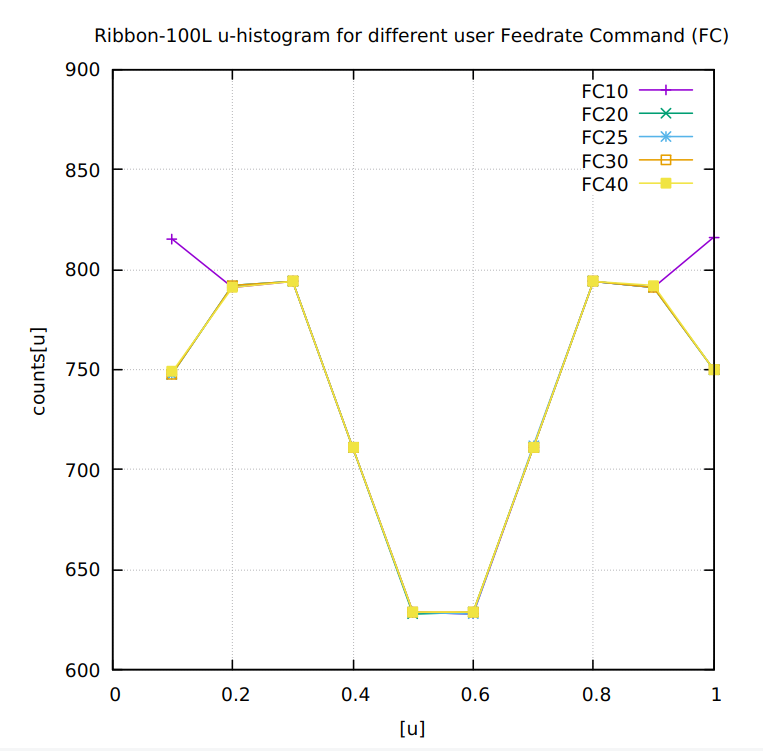
\includegraphics[width=0.95\textwidth]{./07-images/img-Ch54/Img-10-Ribbon-100L-u-histogram.png}}\\
		\end{tabular}
		\caption{Ribbon-100L histogram of interpolated points}		
		\label{table:Ribbon-100L histogram of interpolated points}
	\end{center}
\end{table}
